\chapter{Axioms in Set Theory with Urelements}
In this chapter, I investigate the axiomatization of set theory with urelements. Section \ref{section:additionalaxioms} introduces a group of additional axioms in urelement set theory together with the notion of homogeneity. In Section \ref{section:aHierarchyofAxioms}, I show that the group of axioms form a hierarchy over $\ZFCUR$. This gives rise to a natural question: what is ZFC set theory with urelements? In Section \ref{section:WhatisZFCU}, I present some evidence suggesting that a robust version of ZFC with urelements should include Collection as an axiom. I then consider various philosophical positions one might take regarding this issue. In Section \ref{section:ChoicelesZFU}, I explore urelement set theory without the Axiom of Choice. The hierarchy of axioms in $\ZFCUR$, as I shall prove, largely breaks down when sets of urelements are not necessarily well-orderable.

\section{Additional axioms and homogeneity}\label{section:additionalaxioms}
\subsection{Reflection and dependent choice schemes}
Reflection principles in set theory assert that the set-theoretic universe, $V$, is to some extent indescribable: any statement $\varphi$ will become absolute between some $V_\alpha$ and $V$. In particular, ZF proves the following L\'evy-Montague reflection principle.
\begin{itemize}
    \item [] $\forall \alpha \exists \beta > \alpha\forall x_1, ..., x_n \in V_{\beta} (\varphi(x_1, ..., x_n) \leftrightarrow \varphi^{V_\beta}(x_1, ..., x_n))$.
\end{itemize}
\noindent In urelement set theory, one cannot expect the L\'evy-Montague reflection principle to hold, e.g., if there is a proper class of urelements, then no $V_\alpha(A)$ can reflect such statement for any set of urelements $A$. Instead, in the presence of urelements it should be transitive sets that reflect. Namely,
\begin{itemize}
    \item [] (RP) For every set $x$ there is a transitive set $t$ with $x \subseteq t$ such that for every $x_1, ..., x_n \in t$, $\varphi(x_1, ..., x_n) \leftrightarrow \varphi^t(x_1, ..., x_n)$. \end{itemize}

\begin{prop}\label{RP->Collection}
 ZU + RP $\vdash$ Collection.
\end{prop}
\begin{proof}
First note that RP implies that for any finite collection of formulas $\varphi_1, ..., \varphi_n$, there is a transitive set reflecting each $\varphi_i$. For we can let $\psi(v)$ be the formula $(v=1 \land \varphi_1) \lor ... \lor (v=n \land \varphi_n)$, where $v$ is a new free variable. It follows from RP that there is transitive set $t$ set extending $\omega$ that reflects $\psi(v)$. Consequently, $\varphi_i^t \leftrightarrow \varphi_i$ for each $\varphi_i$. Now suppose that $\forall x \in w \exists y \varphi (x, y, u)$. Let $t$ be a transitive set extending $\{w, u\}$ which simultaneously reflects $\forall x \in w \exists y \varphi (x, y, u)$ and $\varphi(x, y, u)$. It follows that $t$ is a desired collection set. 
\end{proof}
There is another seemingly weaker version of RP, which asserts that any true statement is true in some transitive set containing the parameters.
\begin{itemize}
    \item [] (RP$^-$) If $\varphi (x_1, ..., x_n)$, then there is a transitive set $t$ containing $x_1, ..., x_n$ such that $\varphi^t(x_1, ..., x_n)$.
\end{itemize}
\noindent This form of reflection was first introduced by L\'evy \cite{Levy1966principles}. And in \cite{Levy1961principles} L\'evy and Vaught showed that over Zermelo set theory, RP$^-$ does not imply RP.


The Axiom of Dependent Choice (DC) asserts that for any set $x$, if $r \subseteq x \times x$ is a \textit{set relation} without terminal nodes, then there is an infinite sequence $s \in x^\omega$ such that $\<s(n), s (n+1)> \in r$ for every $n$. DC can be generalized to DC$_\kappa$ for any infinite cardinal $\kappa$ as follows (first introduced by L\'evy in \cite{bwmeta1.element.bwnjournal-article-fmv54i1p13bwm}). 
\begin{itemize}
    \item [] (DC$_\kappa$) For every $x$ and $r\subseteq x \times x$, if for every $s \in x^{<\kappa}$, there is some $w \in x$ such that $\<s, w> \in r$, then there is an $f: \kappa \rightarrow x$ such that $\<f\restriction\alpha, f(\alpha)> \in r$ for all $\alpha < \kappa$.
\end{itemize}
$\ZFCUR$ proves $\forall \kappa$DC$_\kappa$ because we can well-order $x$ and construct the desired function $f$ on $\kappa$ by recursion. What will interest us is the following class version of dependent choice.
\begin{itemize}
    \item [] (DC-scheme) If for every $x$ there is some $y$ such that $\varphi(x, y, u)$, then for every $p$ there is an infinite sequence $s$ such that $s(0) = p$ and $\varphi(s(n), s(n+1), u)$ for every $n<\omega$.
\end{itemize} 

\noindent The DC-scheme says that if $\varphi$ defines a class relation without terminal nodes, then there is an infinite sequence threading this relation. Similarly, we can formulate a class version of DC$_\kappa$ for any infinite cardinal $\kappa$.
\begin{itemize}
        \item[]  (DC$_\kappa$-scheme) If for every $x$ there is some $y$ such that $\varphi(x, y, u)$, then there is some function $f : \kappa\rightarrow U$ such that $\varphi(f\restriction \alpha, f(\alpha), u)$ for every $\alpha <\kappa$.
\end{itemize}
DC$_{<Ord}$ holds just in case the DC$_\kappa$-scheme holds for every $\kappa$. As we shall see, over $\ZFCUR$ the DC$_\kappa$-scheme is strictly stronger than DC$_\kappa$, and in fact, $\ZFCUR$ cannot even prove the DC$_\omega$-scheme. Let us verify that the DC-scheme is indeed a reformulation of the DC$_\omega$-scheme.
\begin{prop}
Over $\ZFUR$, the DC$_\omega$-scheme is equivalent to the DC-scheme.
\end{prop}
\begin{proof}
Assume the DC$_\omega$-scheme and suppose that the relation $\varphi(x, y,u)$ has no terminal nodes. Fix any $p$ and define $\psi(x, y, p, u)$ as follows.
\begin{enumerate}
    \item [] $\psi(x, y, p, u)$ $=_\textup{df}$ $(x = \emptyset \land y = p) \lor \exists n  (x = \langle x_0, ..., x_{n} \rangle \land \varphi (x_n, y, u)) \lor (x \neq \emptyset \land x$ is not a finite sequence$)$
\end{enumerate}
Since $\psi(x, y, p, u)$ has no terminal nodes, there is a function $f$ on $\omega$ such that $\psi(f\restriction n, f(n), p, u)$ for all $n$. It then follows that $f(0) = p$ and $\varphi(f(n), f(n+1), u)$ for all $n$.

Now assume the DC-scheme and suppose that $\varphi(x, y,u)$ has no terminal nodes. Fix some $p$ be such that $\varphi(\emptyset, p, u)$. Let $\psi(x, y, p, u)$ be the formula asserting that either $x$ is not a finite sequence, or $x = \emptyset$ and $y = \<p>$, or for some $n > 0$, $x$ is an $n$-sequence and $y$ is an $n+1$-sequence extending $x$ such that $\varphi(x, y(n), u)$. As $\psi(x, y, p, u)$ has no terminal nodes, it follows that there is an $\omega$-sequence $s$ such that $s(0)= \emptyset$ and $\psi(s(n), s(n+1), p, u)$ for every $n$. Let $f(n) = s(n+1)(n)$. Then $\varphi(f\restriction n, f(n), u)$ for every $n$.
\end{proof}

\begin{prop}\label{prop:DCkappaVariants}
Over $\ZFUR$, for every cardinal $\kappa$, the following are equivalent.
\begin{enumerate}
    \item DC$_\kappa$-scheme. 
    \item For every definable class $X$ and $u$, if every $s \in X^{<\kappa}$ has some $y \in X$ such that $\varphi(x, y, u)$, then there is a function $f \in X^{\kappa}$ such that $\varphi(f\restriction \alpha, f(\alpha), u)$ for every $\alpha < \kappa$. 
\end{enumerate}
\end{prop}
\begin{proof}
(2) $\rightarrow$ (1) is immediate. To show (1) $\rightarrow$ (2), assume (1) and the antecedent of (2). Define
\begin{itemize}
    \item []  $\psi(x, y, u) =_\textup{df} x \in X^{<\kappa} \rightarrow \varphi(x, y, u) \land y \in X.$
\end{itemize}
Then there is an $f : \kappa \rightarrow U$ such that $\psi(f\restriction \alpha, f(\alpha), u)$ for every $\alpha < \kappa$. Consider any $\alpha < \kappa$ and suppose that for every $\beta < \alpha$, $f(\beta) \in X$. Then $f(\alpha) \in X$. So $f\restriction \alpha \in X$ for every $\alpha <\kappa$. Thus, $f \in X^\kappa$  and $\varphi(f\restriction\alpha, f(\alpha), u)$ for every $\alpha < \kappa$.\end{proof}
\begin{theorem}[\cite{Gitman2016-GITWIT}]\label{collection+dc->rp}
$\ZFUR +$ DC$_\omega$-scheme + Collection $\vdash$ RP.
\end{theorem}
\begin{proof}
This is first proved in \cite{Gitman2016-GITWIT} in context of ZFC without Powerset, and the point here is that their argument works in $\ZFUR$. Fix a set $w$ and a formula $\varphi(v_1, ..., v_m)$ and let $\varphi_1, ..., \varphi_n$ be all the subformulas of $\varphi$.  For any set $x$ and $y$, we say that $y$ is a $\varphi$-cover of $x$ if (i) $y$ is transitive and $x \subseteq y$, and (ii) for each $1 \leq i \leq n$,  $\forall x_1, ..., x_m \in x \ [\exists v \varphi_i (v, x_1, ..., x_m) \rightarrow \exists v \in y\  \varphi_i (v, x_1, ..., x_m)]$.

Let us construct a $\varphi$-cover for an arbitrary set $x$. For each $1 \leq i \leq n$, define $z_i = \{s \in x^{<\omega}: \exists v \exists x_1, ..., x_m \in x (\varphi_i (v, x_1, ..., x_m) \land s = \langle x_1, ..., x_{m} \rangle)\}$. For each $ i \leq n$, by Collection there is a $y_i$ such that for every $s \in z_i$, there is $v \in y_i$ such that  $\exists x_1, ..., x_m \in x [\varphi_i (v, x_1, ..., x_m) \land s = \langle x, ..., x_m \rangle]$. Set $y = trc(\bigcup_{i\leq n} y_i \cup x)$. $y$ is then a $\varphi$-cover of $x$. Thus, by the DC$_\omega$-scheme, there is an $\omega$-sequence $\langle z_n : n< \omega \rangle$ such that $z_0 = w$ and $z_{n+1}$ is a $\varphi$-cover of $z_n$ for every $n$. Set $t = \bigcup_{n < \omega} z_n$. By a routine induction on the subformulas of $\varphi$, it follows that for every $x_0, ..., x_m \in t$, $\varphi^t (x_1, ..., x_m) \leftrightarrow \varphi (x_1, ..., x_m)$.
\end{proof}

\subsection{Urelement axioms and homogeneity}
\begin{definition}
A set $x$ is \textit{realized} if there is a set of urelements equinumerous with $x$. Let $A$ be a set of urelements.
\begin{enumerate}
    \item A set of urelements $B$ \textit{duplicates} $A$, if $B$ and $A$ are disjoint and equinumerous.
    \item A set of urelements $B$ is a \textit{tail} of $A$, if $B$ is disjoint from $A$ and for every $C \subseteq \A$ disjoint from $A$ there is an injection from $C$ to $B$.
    \item \textit{Duplication holds over} $A$, if every $B \subseteq \A$ disjoint from $A$ has a duplicate $C$ that is also disjoint from $A$;
    \item \textit{Homogeneity holds over} $A$, if whenever $B$ and $C$ are equinumerous and $B \cup C \subseteq \A$ is disjoint from $A$, there is an automorphism $\pi$ such that $\pi B = C$ and $\pi$ point-wise fixes $A$.
\end{enumerate}
\end{definition}
\noindent Intuitively, when homogeneity holds over $A$, the urelements outside $A$ are all indistinguishable from the perspective of $A$. We shall consider the following axioms.
\begin{enumerate}
    \item [] (Plenitude) Every cardinal is realized.
    \item [] (Closure) The supremum of a set of realized cardinals is realized.
    \item [] (Duplication) Every set of urelements has a duplicate.
    \item [] (Tail) Every set of urelements has a tail.
    \item [] ($\ACA$) Every set of urelements is well-orderable.
\end{enumerate}
$\ACA$ is strictly weaker than AC over $\ZFUR$ even if we assume there are infinitely many urelements: let $V$ be a model of ZF $+$ $\neg$AC and consider $V\llbracket Ord \rrbracket$ (Definition \ref{barwiseinterpretation1}); by Theorem \ref{thm:ACholdsViffACholdsinV[X]}, $V\llbracket Ord \rrbracket \models \ACA \land \neg$AC. With $\ACA$, Tail is equivalent to the following.
\begin{itemize}
    \item [] (Tail$^*$) For every $A \subseteq \A$, there is a greatest cardinal $\kappa$ such that $\exists B \subseteq \A \ (B \sim \kappa \land B \cap A = \emptyset)$,
\end{itemize}
where $\kappa$ is called the \textit{tail cardinal} of $A$.
\begin{lemma}[$\ZFUR$]\label{homogeneitylemma}
\ 
\begin{enumerate}
    \item If $A \subseteq A' \subseteq \A$ and duplication holds over $A$, then duplication holds over $A'$.
    \item If duplication holds over $A \subseteq \A$, then homogeneity holds over $A$.
    \item Assume Tail and $\ACA$. Duplication holds over some set of urelements.%Tail alone does not suffice. See the model where Tail holds and Collection fails.%
    \item Assume $\ACA$. For every $A \subseteq \A$, there is an $A' \subseteq \A$ such that $A \subseteq A'$ and duplication (hence homogeneity) holds over $A'$.
\end{enumerate}
\end{lemma}
\begin{proof}
(1) If $B$ is disjoint from $A'$, then there is another $C$ disjoint from $A$ that is equinumerous with $(A'\setminus A) \cup B$. So $C$ contains a duplicate of $B$ that is disjoint from $A'$.

(2) This is first proved in \cite{HamkinsForthcoming-HAMRIS}. Let $B$ and $C$ be such that $B \sim C$ and $B \cup C$ is disjoint from $A$. If $B$ and $C$ are duplicates, then by swapping them we can get a permutation $\pi$ with $\pi B = C$ that point-wise fixes $A$. If not, then by duplication over $A$, there is a duplicate of $B \cup C$ disjoint from $A \cup B \cup C$ and hence a duplicate $D$ of both $B$ and $C$ that is disjoint from $A$. Thus, there are automorphisms $\pi_1$ and $\pi_2$ such that $\pi_1 B = D$ and $\pi_2 D = C$, and both of them point-wise fix $A$. The composition of $\pi_1$ and $\pi_2$ is the desired automorphism.

(3) Assume Tail and $\ACA$. Let $\kappa$ be the least cardinal that is a tail cardinal of some $D \subseteq \A$. If $B$ is disjoint from $D$, since the tail cardinal of $D \cup B$ is at least $\kappa$, there is another $C$ disjoint from $D \cup B$ that has size at least $\kappa$. Since $B$ is well-orderable and hence has size at most $\kappa$, $C$ contains a duplicate of $B$. Therefore, duplication holds over $D$.

(4) Assume $\ACA$. By (1) and (2), it suffices to show that duplication holds over some set of urelements. Suppose otherwise. Then $\A$ is a proper class, and by (3), some $A \subseteq \A$ has no tail cardinal. Given any infinite $B$ disjoint from $A$, since $B$ is equinumerous with some cardinal $\kappa$, there must be some $C$ of size $\kappa^+$ that is disjoint from $A$. But then C contains a duplicate of $B$ . This shows that duplication holds over $A$ after all, which is a contradiction.
\end{proof}
\noindent In general, homogeneity does not imply duplication: if $\A$ is a set and $\A \setminus A$ has only one urelement, then duplication does not hold over $A$ while homogeneity holds over $A$ trivially. And assuming $\ACA$, duplication holds over $A$ if homogeneity holds over $A$ and $\A \setminus A$ is not a finite non-empty set. To see this, let $B$ be a set of urelements disjoint from $A$, and we may assume $B$ is infinite. By $\ACA$, $B$ can be partitioned into a pair of duplicates $B_1$ and $B_2$. By homogeneity over $A$, there is an automorphism $\pi$ such that $\pi B_1 = B$ and $\pi A =A$. Since $B_1$ has a duplicate disjoint from $A$, it follows that $B$ has one too and hence duplication holds over $A$. In Section \ref{section:ChoicelesZFU}, I will show that $\ACA$ is necessary for homogeneity to hold over some set of urelements. In particular, there are models of $\ZFUR$ + RP + DC$_\omega$-scheme where homogeneity holds over no set of urelements.



\section{A hierarchy of axioms in $\ZFCUR$}\label{section:aHierarchyofAxioms}

\subsection{Implication diagram in $\ZFCUR$}\label{subsection:implicationdiagram}
The main theorem of this section is the following.
\begin{theorem}\label{maintheorem1}
Over $\ZFCUR$, the following implication diagram holds. Moreover, the diagram is complete: if the diagram does not indicate $\varphi$ implies $\psi$, then $\textup{ZFCU}_\text{R}$ $+$ $\varphi \nvdash \psi$ assuming the consistency of ZF.
\end{theorem}
\begin{figure}[hbt!]
\begin{center}
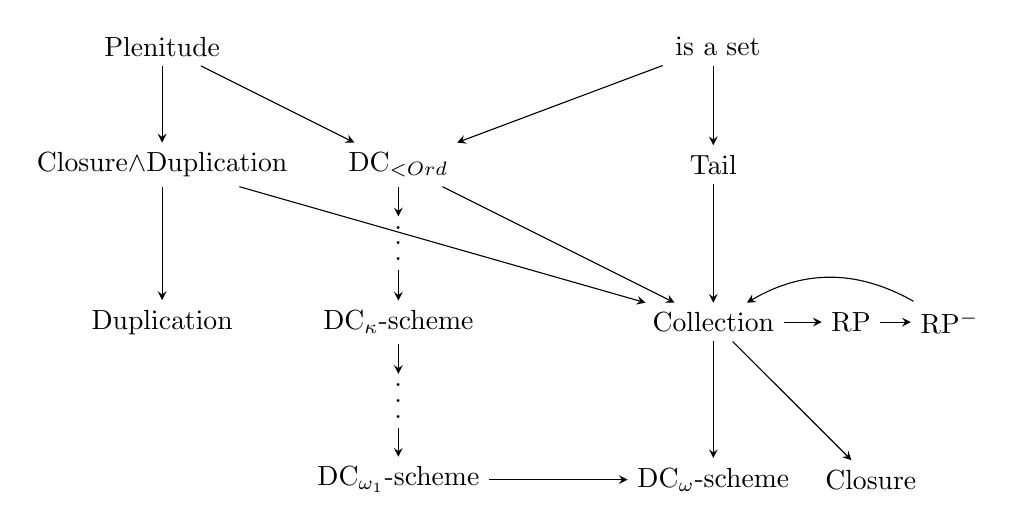
\begin{tikzpicture}
\begin{scope}[every node/.style={}]
    \node (A) at (10, -2.5) {DC$_\omega$-scheme};
    \node (B) at (10, 1.5){Tail};
    \node (C) at (3,3) {Plenitude};
     \node (D) at (6,1.5) { DC$_{<Ord}$ };
    \node (E) at (6, -0.5) {DC$_\kappa$-scheme};
       \node (F) at (12, -2.5) {Closure};
          \node (G) at (11.75, -0.5) {RP};

    \node (H) at (3, 1.5) {\textup{Closure$\land$Duplication}};
    \node (I) at (10, -0.5) {Collection};
        \node (J) at (13, -0.5) {RP$^-$};

    \node (L) at (6, 0.7) {.};
    \node (M) at (6, 0.5) {.};
    \node (N) at (6, 0.3) {.};
    \node (O) at (3, -0.5) {Duplication};
    \node (P) at (6, -1.7) {.};
    \node (Q) at (6, -1.5) {.};
    \node (R) at (6, -1.3) {.};
    \node (S) at (6, -2.5) {DC$_{\omega_1}$-scheme};
    \node (T) at (10, 3) {$\A$ is a set};
    
\end{scope}

\begin{scope}[>={stealth},
              every node/.style={fill=white,circle},
              every edge/.style={draw=black}]
 
    \path [->] (T) edge (B);
    \path [->] (T) edge (D);
    \path [->] (C) edge (H);
    \path [->] (B) edge (I);
    \path [->] (I) edge (A);

     \path [->] (S) edge (A);


    \path [->] (H) edge (I);
    \path [->] (H) edge (O);
    
     \path [->] (C) edge (D);

    \path [->] (D) edge (I);
    \path [->] (D) edge (L);
    \path [->] (N) edge (E);
    \path [->] (E) edge (R);
     \path [->] (P) edge (S);
    
    \path [->] (I) edge (F);

    \path [->] (I) edge (G);
   \path [->] (G) edge (J);
   
       \path [->] (J) edge[bend right=30] (I); 
\end{scope}
\end{tikzpicture}
 \caption{Implication diagram in $\ZFCUR$}
 \label{ZFCUdiagram}
\end{center}
\end{figure}
\FloatBarrier
\noindent The direction from Collection to the DC$_\omega$-scheme was first proved by Schlutzenberg in an answer to a question on Mathoverflow \cite{387471} and the notion of tail cardinal was also implicit in his proof (\cite{HamkinsForthcoming-HAMRIS} also contains a different proof of Collection $\rightarrow$ DC$_\omega$-scheme). My proof of Collection $\rightarrow$ DC$_\omega$-scheme takes a different route and appeals to a key observation that Tail implies Collection, which will also be crucial for later discussions.


The rest of this subsection establishes the implication diagram, while the next subsection proves its completeness. Let us first show that Plenitude implies DC$_{<Ord}$. Given a formula $\varphi(x, y, u)$ with a parameter $u$, for any ordinals $\alpha, \alpha', \kappa, \kappa'$ and a set of urelements $E$, we say that $\<\kappa' \alpha'>$ is a $(\varphi, E)$\textit{-extension} of $\<\kappa, \alpha>$ if (i) $\alpha \leq \alpha'$, and (ii) whenever $A \subseteq \A$ extends $E$ by $\kappa$-many urelements, there is some $B \subseteq \A$ disjoint from $A$ with $B \sim \kappa'$ such that for every $x \in V_{\alpha}(A)$, there is some $y \in V_{\alpha'} (A \cup B)$ such that $\varphi (x, y, u)$. 
\begin{lemma}($\ZFCUR$)\label{phiextension}
Suppose that Plenitude holds and $\varphi(x, y, u)$ defines a relation without terminal nodes. Then every $\langle \kappa, \alpha \rangle$ has a $(\varphi, ker(u))$-extension.
\end{lemma}
\begin{proof}
First note that under $\ZFCUR$ + Plenitude, homogeneity holds over every set of urelements. Fix$\langle \kappa, \alpha \rangle$ and some $A \subseteq \A$ extending $ker(u)$ with $\kappa$-many urelements. For each $x\in V_\alpha(A)$, define $\theta_x$ to be the least cardinal such that there is some $y$ with $\varphi(x, y, u)$ and $ker(y) \sim \theta_x$, and let $\kappa' = Sup\{ \theta_x : x \in  V_\alpha(A)\}$. Fix some infinite $B$ of size $\kappa'$ that is disjoint from A, which exists by Plenitude. Then for every $ x \in V_\alpha(A)$, fix some $y'$ such that $\varphi(x, y', u)$ and $ker(y') \sim \theta_x$. $ker(y') \setminus A$ is equinumerous to a subset of $B$, so by homogeneity over $A$, there is an automorphism $\pi$ that moves $ker(y')$ into $B$ and point-wise fixes $A$. It follows that $\varphi(x, \pi y', u)$ and $\pi y' \in V(A \cup B)$. Thus, each $x \in V_\alpha(A)$ has some $y \in V(A\cup B)$ with $\varphi(x, y, u)$, so there is some large enough $\alpha'$ such that every $x \in V_\alpha(A)$ has some $y \in V_{\alpha'}(A\cup B)$ with $\varphi(x, y, u)$. Furthermore, for every $A'$ extending $ker(u)$ by $\kappa$-many urelements, by homogeneity over $ker(u)$, there is an automorphism $\pi$ with $\pi A = A'$ that point-wise fixes $\ker(u)$; so $\pi B$ will be such that every $x \in V_\alpha(A')$ has some $y \in V_{\alpha'}(A' \cup \pi B)$ with $\varphi(x, y, u)$. Therefore, $\<\kappa', \alpha'>$ is indeed a $(\varphi, ker(u))$-extension of $\<\kappa, \alpha>$.
\end{proof}








\begin{theorem}\label{Plenitude->DCS}
 $\ZFCUR$ $\vdash$Plenitude $\rightarrow$ DC$_{<Ord}$.
\end{theorem}
\begin{proof}
Suppose that Plenitude  holds and  $\varphi(x, y, u)$ defines a relation without terminal nodes with some parameter $u$. Consider any infinite cardinal $\kappa$. To prove the DC$_\kappa$-scheme, we first find a set $\barx$ that is closed under $<\kappa$-sequences and the relation $\varphi$; we can then apply DC$_\kappa$ to get a desired function on $\kappa$. Let $\delta$ be a cardinal with $\textup{cf}(\delta) = \kappa$. We first define a $\delta$-sequence of pairs of ordinals $\langle \langle \lambda_\alpha, \gamma_\alpha \rangle : \alpha < \delta \rangle$ by recursion as follows. Let $A_0$ be a set of urelements that extends $\ker(u)$ by $\lambda_0$-many urelements and $\gamma_0$ be an ordinal with cf$(\gamma_0)  \geq \kappa$. For each ordinal $\alpha < \delta$, we let $\langle \lambda_{\alpha+1} , \gamma_{\alpha+1} \rangle$ be the lexicographical-least $(\varphi, ker(u))$-extension of $\<\lambda_\alpha ,\gamma_\alpha>$ with cf$(\gamma_\alpha) \geq \kappa$, which exists by the previous lemma. And we take the union at the limit stage.


By Plenitude, we can fix a $\delta$-sequence of sets of urelements $\langle A_\alpha : \alpha < \delta \rangle$, where $A_\alpha$ extends $\bigcup_{\beta < \alpha} A_\beta \cup ker(u)$ by $\lambda_\alpha$-many urelements. Let $\barx = \bigcup_{\alpha < \delta} V_{\gamma_\alpha} (A_\alpha)$. For any $x \in V_{\gamma_\alpha} (A_\alpha)$, There is some $B$ disjoint from $A_\alpha$ witnessing the fact that $\<\lambda_{\alpha +1}, \gamma_{\alpha+1}>$ is a $(\varphi, ker(u))$-extension of $\<\lambda_\alpha ,\gamma_\alpha>$. And by homogeneity over $A$, it follows that $A_{\alpha +1} \setminus A_\alpha$ works as such witness as well; so there is some $y \in V_{\gamma_{\alpha +1}}(A_{\alpha +1})$ with $\varphi(x, y, u)$, and such $y$ lives in $\barx$. $\barx$ is also closed under $<\kappa$-sequences since $\textup{cf}(\delta) = \kappa$ and each $V_{\gamma_\alpha} (A_\alpha)$ is closed under $<\kappa$-sequences. Thus, if $s \in \barx^{<\kappa}$, there is some $y \in \barx$ such that $\varphi (s, y, u)$. By DC$_\kappa$, there exists a function $f$ on $\kappa$ such that $\varphi (f\restriction \alpha, f(\alpha), u)$ for all $\alpha < \kappa$. Hence, the DC$_\kappa$-scheme holds.
\end{proof}


\begin{lemma} \label{Plenitude->Collection}
$\ZFUR + \ACA$ $\vdash$ Closure $\land$ Duplication $\rightarrow$ Collection
\end{lemma}
\begin{proof}
Fix some set $w$ such that $\forall x \in w \exists y \varphi (x, y, u)$. For every $x \in w$, let $\theta_x$ be the least $\theta$ realized by the kernel of some $y$ such that $\varphi(x, y, u)$, and define $\theta$ as the supremum of all such $\theta_x$. Let $A \subseteq \A$ be such that $ker(w) \cup \ker(u) \subseteq A$ and duplication holds over $A$,  which exists by Lemma \ref{homogeneitylemma} (4). By Closure and Duplication, there is a $B \subseteq \A$ of size $\theta$ that is disjoint from $A$. Then for every $x \in w$, fix a $y'$ such that $\varphi(x, y', u)$ with the smallest kernel. By homogeneity over $A$, there is an autormophism that moves $ker(y')$ into $A \cup B$ without moving any urelements in $A$. Therefore, every $x \in w$ has a $y \in V(A \cup B)$ such that $\varphi(x, y, u)$. Then Collection holds by applying Proposition \ref{weakcollection}.
\end{proof}

\begin{lemma}\label{tail->collection}
$\ZFUR + \ACA$ $\vdash$ Tail $\rightarrow$ Collection
\end{lemma}
\begin{proof}
Assume that every set of urelements has a tail. Suppose that every $x \in w $ has some $y$ with $\varphi (x, y, u)$. Let $A \subseteq \A$ be such that $ker(w) \cup ker(u) \subseteq A$ and duplication holds over $A$ and $B$ be a tail of $A$. For every $x \in w$ and $y$ such that $\varphi(x, y, u)$, $B$ must contain a subset that is equinumerous with $ker(y) \setminus A$. By homogeneity over $A$, there is an automorphism that moves $ker(y)$ into $A \cup B$ while point-wise fixing $A$. Therefore, every $x \in w$ has some $y \in V(A \cup B)$ such that $\varphi (x, y, u)$ and hence Collection holds by Proposition \ref{weakcollection}.
\end{proof}

\begin{lemma}[$\ZFCUR$]\label{Tailkappa->DCkappa}
Let $\kappa$ be an infinite cardinal and suppose that every set of urelements has a tail of size at least $\kappa$. Then the DC$_\kappa$-scheme holds.
\end{lemma}
\begin{proof}
First assume that $\kappa$ is regular. Suppose that $\varphi(x, y, u)$ defines a relation without terminal nodes with a parameter $u$. Let $A$ be a set of urelements extending $ker(u)$ over which duplication holds and $B$ be a tail of $A$. Since $B$ has size at least $\kappa$, $B$ can be partitioned into $\kappa$-many pieces $\{B_\eta : \alpha < \kappa\}$, where each $B_\eta$ is equinumerous with $B$. Let $\beta$ be a ordinal such that cf$(\beta) = \kappa$. We define a $\kappa$-sequence of ordinals $\<\gamma_\alpha : \gamma < \kappa>$ above $\beta$ by recursion, where $\gamma_\alpha$ is the least ordinal such that 
\begin{itemize}
    \item [] (i) $\gamma_\alpha > \bigcup_{\eta < \alpha} \gamma_\eta$ and cf$(\gamma_\alpha) = \kappa$;
    \item [] (ii) for every $x$ in $ \bigcup_{\eta < \alpha} V_{\gamma_\eta}(\bigcup_{\eta < \alpha}B_\eta \cup A)$, there is a $y \in V_{\gamma_\alpha}(\bigcup_{\eta \leq \alpha} B_\eta \cup A)$ with $\varphi(x, y, u)$.
\end{itemize}
Such $\gamma_\alpha$ exists because homogeneity holds over $\bigcup_{\eta < \alpha}B_\eta \cup A$ and each $B_\alpha$ is a tail of of $A$. Let $x = \bigcup_{\alpha < \kappa} V_{\gamma_\alpha}(\bigcup_{\eta \leq \alpha}B_\eta \cup A)$. $x$ is then closed under $\varphi(x, y, u)$. And since $x$ is the union of an increasing $\kappa$-sequence of sets and each $\gamma_\alpha$ has cofinality $\kappa$, it follows that $x^{<\kappa} \subseteq x$. We can then apply DC$_\kappa$ to $x$ to get a desired $\kappa$ sequence, so the DC$_\kappa$-shceme holds.

Suppose $\kappa$ is singular. Then for every regular $\lambda < \kappa$, the argument in the previous paragraph shows that the DC$_\lambda$-scheme holds. But this implies the DC$_\kappa$-scheme by a standard argument as in \cite[Theorem 8.1]{jech2008axiom}.
\end{proof}

\noindent To show that Diagram \ref{ZFCUdiagram} holds, it remains to prove the following.

\begin{lemma}\label{easyimplication}Over $\ZFCUR$, the following implications hold.
\begin{enumerate}
    \item $\mathcal{A}$ is a set $\rightarrow$ DC$_{<Ord}$. 
    \item DC$_{<Ord}$ $\rightarrow$ Collection
    \item RP$^-$ $\rightarrow$ Collection.
    \item Collection $\rightarrow$ Closure
    \item Collection $\rightarrow$ DC$_\omega$-scheme.
    \item Collection $\rightarrow$ RP.
\end{enumerate}
\end{lemma}
\begin{proof}



(1) This is proved by a standard argument, which I include for completeness. Assume $\mathcal{A}$ is a set and $\forall x \exists y \varphi (x, y, u)$. Fix any $\kappa$ and let $\delta$ be such that cf$(\delta)= \kappa$. We define a $\delta$-sequence of ordinals $\langle \gamma_\alpha : \alpha < \delta \rangle$, where $\gamma_\alpha$ is the least ordinal of cofinality $\kappa$ such that $\forall x \in \bigcup_{\eta <  \alpha} V_{\gamma_\eta} (\mathcal{A}) \exists y \in V_{\gamma_\alpha}(\mathcal{A}) \varphi (x, y, u)$. Then the DC$_\kappa$-scheme holds by applying DC$_\kappa$ to $\bigcup_{\alpha < \delta} V_{\gamma_\alpha} (\mathcal{A})$.

(2) This is because under DC$_{<Ord}$, either $\A$ is a set or Plenitude holds, but Collection holds either way by Proposition \ref{weakcollection} and Lemma \ref{Plenitude->Collection}.

(3) Suppose that RP$^-$ holds. It suffices to show that Tail holds by Lemma \ref{tail->collection}. We may assume that  $\mathcal{A}$ is not a set and Plenitude fails by Lemma \ref{Plenitude->Collection}.  Fix some $A \subseteq \A$ and let $\kappa$ be the least cardinal not realized by some $B \subseteq \A$ that is disjoint from $A$. Then there is a transitive set $t$ reflecting the statement that $\forall \lambda < \kappa \exists B (B \sim \lambda \land B \cap A = \emptyset )$. We may assume that $t$ extends $\{\kappa, A\}$ and is closed under pairs. $C = \bigcup \{B \in t : B \subseteq \A \land B \cap A = \emptyset\}$ is then a tail of $A$.

Now assume Collection. 

(4) Let $x$ be a set of realized cardinals. Then there is a set $y$ such that for every $\kappa \in x$, there is some $A \in y$ such that $A \sim \kappa$. Let $B = \bigcup \{A: A \in y\}$. Then the cardinality of $B$ is at least the supremum of $x$ and hence Closure holds. 

(5) Observe that Collection + $\neg$Plenitude implies Tail. Given a set $A$ of urelements, let $w$ be the set of cardinals realized by some $B \subseteq \A$ disjoint from $A$. Then there is some $v$ such that for every $\lambda \in w$, there is some $B \in v$ such that $B \sim \lambda$ and $B \cap A = \emptyset$. $C = \bigcup \{B \in v: B \cap A = \emptyset\}$ is then a tail of $A$. Now to show the DC$_{\omega}$-scheme holds, we may assume that Plenitude fails by Theorem \ref{Plenitude->DCS}. Then every set of urelements must have an infinite tail, so the DC$_{\omega}$-scheme follows from Lemma \ref{Tailkappa->DCkappa}.

(6) RP holds by (5) and Theorem \ref{collection+dc->rp}.
\end{proof}


\subsection{Independence results}
I now proceed to show that Diagram \ref{ZFCUdiagram} is complete by an easy method of building inner models of $\ZFCUR$, which was implicitly used in \cite{levy1969definability} and \cite{felgner1976choice}.
 \begin{definition}[$\ZFUR$]\label{normalideal}
A (definable) class $\I$ of sets of urelements is an $\A$-\textit{ideal} if 
\begin{enumerate}
    \item $\A \notin \I$ (if $\A$ is a set);
    \item if $A, B \in \I$, then $A \cup B \in \I$; 
    \item if $A \in \I$ and $B \subseteq A$, then $B \in \I$;
    \item for every $a \in \A$, $\{a\} \in \I$.
\end{enumerate}
Given an $\A$-ideal $\I$, $U^\I = \{x \in U : ker(x) \in \I\}$, i.e., the class of objects whose kernel is in $\I$.
 \end{definition}
 

\begin{lemma}[$\ZFUR$]\label{idealpermutation}
Let $\I$ be an $\A$-ideal. Then for every $a, A$ such that $a \in A \in \I$, there is a permutation $\pi$ of $\mathcal{A}$ such that (i) $\pi \I = \I$, (ii) $\pi a \neq a$ and (iii) $\pi$ point-wise fixes $A \setminus \{a\}$.
\end{lemma}
\begin{proof}
Fix some $a^* \in \mathcal{A} \setminus A$. Let $\pi$ be a permutation that only swaps $a$ and $a^*$. To see that $\pi \I = \I$, let $B \in \I$. Without lost of generality, we may assume $a \in B$ and $a^* \notin B$. Then $\pi B = (B \setminus \{a\}) \cup \{a^*\}$, which is in $\I$. Also, $B = \pi ((B \setminus \{a\}) \cup \{a^*\})$. Therefore, $\pi \I = \I$.
\end{proof}

\begin{theorem}[$\ZFUR$]\label{smallkernelmodel}
Let $\I$ be an $\A$-ideal.
\begin{enumerate}
\item $U^\I \models \ZFUR$ + ``$\A$ is a proper class'';
\item $U^\I \models $ AC if $U \models $ AC.
\end{enumerate}
\end{theorem}
\begin{proof}
It is clear that $U^\I$ is transitive and contains all the urelements and pure sets. Thus, $U^\I$ satisfies Foundation, Extensionality, Infinity, and $\A$ is a proper class in  $U^\I$. It is also immediate that $U^\I$ satisfies Pairing, Union, Powerset and Separation. When AC holds in $U$, it holds in $U^\I$ because for a given set $x$ in $U^\I$, any bijection in $U$ between $x$ and an ordinal has the same kernel as $x$ and hence also lives in $U^\I$. It remains to show that Replacement holds in $U^\I$.

Suppose that $U^\I \models \forall x \in w \exists ! y \varphi (x, y, u)$ for some $w, u \in U^\I$. Let $v = \{ y \in U^\I : \exists x \in w\ \varphi^{U^\I}(x, y, u) \}$, which is a set in $U$. It suffices to show that $ker(v) \subseteq  ker(w) \cup ker(u)$. Suppose not. Then there are some $y$ and $a$ such that $y \in v$, $a \in ker(y)$\footnote{Note that by our convention (Definition \ref{def:kernel,cardinal}) if $y$ is an urelement, $ker(y) = \{y\}$.} and $a \notin ker(w) \cup ker(u)$. Let $A = ker(w) \cup ker(u) \cup ker(y)$, which is in $\I$. By Lemma \ref{idealpermutation}, there is an automorphism $\pi$ such that (i) $\pi \I = \I$, (ii) $\pi a \neq a$ and (iii) $\pi$ point-wise fixes $A \setminus \{a\}$. So $\pi$ point-wise fixes $w$ and $u$. Since $y \in v$, there is some $x \in w$ with $\varphi^{U^\I}(x, y, u)$. It follows that $\varphi^{U^\I}(x, \pi y, u)$, but $\pi y \neq y$ because $\pi a$ is in $ker(\pi y)$ but not in $ker(y)$, which contradicts the uniqueness of $y$.
\end{proof}


\begin{theorem}\label{zfcurindependece}
Assume the consistency of ZF. Over $\ZFCUR$,
\begin{enumerate}
     \item (Closure $\land$ Duplication) $\nrightarrow$ (Plenitude $\lor$ DC$_{\omega_1}$-scheme);
    \item  Collection $\nrightarrow$ Duplication;
    \item  Duplication $\nrightarrow$ (Closure $\lor$ DC$_\omega$-scheme);
    \item  Closure $\nrightarrow$ DC$_\omega$-scheme;
    \item  DC$_\kappa$-scheme $\nrightarrow$ Closure, where $\kappa$ is any infinite cardinal;
    \item (Collection $\land$ DC$_\kappa$-scheme) $\nrightarrow$ DC$_\lambda$-scheme, where $\kappa < \lambda$ are infinite cardinals.
\end{enumerate}
Hence, Diagram \ref{ZFCUdiagram} is complete.
\end{theorem}
\begin{proof}
In each case, $U$ is a model of $\ZFCUR$. These models exist if ZF is consistent by Theorem \ref{con(zfc)->con(zfcu)}.

(1) Assume that in $U$, $\mathcal{A} \sim \omega_1$. Let $\I_1$ be the ideal of all countable subsets of $\mathcal{A}$. In $U^{\I_1}$, $\omega$ is the greatest realized cardinal. It is clear that Closure Duplication hold while Plenitude fails. The DC$_{\omega_1}$-scheme fails in $U^{\I_1}$ because every kernel can be properly extended but there cannot be a function $f$ on $\omega_1$ such that $ker(f\restriction \alpha) \subsetneq ker(f(\alpha))$ for all $\alpha < \omega_1$, as the kernel of such $f$ would be uncountable.  

(2) Assume that in $U$, $\mathcal{A} \sim \omega_1$. Fix an $A \subseteq \A$ such that $A \sim \omega_1$ and $\A \setminus A \sim \omega_1$. Let $\I_2 = \{ B \subseteq \mathcal{A}:  B  \setminus A \text{ is countable} \}$. For every $B \in U^{\I_2}$, let $\lambda =$Max$\{|A \setminus B|, \omega\}$, where $|A\setminus B|$ is the cardinality of $A\setminus B$. $\lambda$ is then the tail cardinal of $B$. So Collection holds in $U^{\I_2}$ by Lemma \ref{tail->collection}. Duplication fails because $A$ has no duplicates in $U^{\I_2}$.

(3) Assume that in $U$, $\mathcal{A} \sim \omega$. Let $\I_3$ be the ideal of finite subsets on $\mathcal{A}$. It is cleat that in $U^{\I_3}$ Duplication holds and Closure fails. The DC$_\omega$-scheme also fails in $U^{\I_3}$ because set of urelements can be properly extended but there is no infinite increasing sequence of sets of urelements.

(4) Assume that in $U$, $\mathcal{A} \sim \omega$ and fix an infinite and co-infinite $A \subseteq \A$. Let $\I_4 = \{ B \subseteq \mathcal{A}: B \setminus A \text{ is finite}\}$. Closure holds in $U^{\I_4}$ because $\omega$ is the greatest realized cardinal. The DC$_\omega$-scheme fails in $U^{\I_4}$ since every set of urelements can be properly extended by another set of urelements disjoint from $A$. but there cannot be a corresponding infinite sequence.

(5) Let $\kappa$ be an infinite cardinal. Assume that in $U$, $\mathcal{A} \sim \omega_{\kappa^+}$. Let $\I_5$  be the set of sets of urelements of size less than $\omega_{\kappa^+}$. Closure fails in $U^{\I_5}$ because $ \omega_{\kappa^+}$ is not realized while every cardinal below it is realized. To show that the DC$_\kappa$-scheme holds, suppose that for every $x \in U^{\I_5}$, there is some $y \in U^{\I_5}$ such that $\varphi^{U^{\I_5}}(x, y, u)$. $U^{\I_5}$ is closed under $\kappa$-sequences. Since DC$_{<Ord}$ holds in $U$ by Lemma \ref{easyimplication}, in $U$ there is a function $f: \kappa \rightarrow U^{\I_5}$ such that $\varphi^{U^{\I_5}}(f\restriction\alpha, f(\alpha), u)$ for every $\alpha < \kappa$, and $f$ lives in $U^{\I_5}$.

(6) It suffices to show that for any $\kappa$, $\ZFCUR$ + Collection + the DC$_\kappa$-scheme does not prove the DC$_{\kappa^+}$-scheme. Assume that in $U$, $\A \sim \kappa^+$ and let $\I_6$ be the ideal of all sets of urelements of size less than $\kappa^+$. By an argument as before, the DC$_{\kappa^+}$-scheme fails in $U^{\I_6}$. Every set of urelements in $U^{\I_6}$ has tail cardinal $\kappa$, so Collection holds by Lemma \ref{tail->collection} and the DC$_\kappa$-scheme holds by Lemma \ref{Tailkappa->DCkappa}.
\end{proof}
Combining the $U^\I$-construction with the $V\llbracket X \rrbracket$-construction in Definition \ref{barwiseinterpretation1}, we can further establish the mutual interpretability between various extensions of $\ZFCUR$.
\begin{corollary}\label{zfcumutualinter}
 The following theories are pairwise mutually interpretable.  
 \begin{enumerate}
     \item $\ZFCUR$ + Plenitude + $\neg$CH.
     \item $\ZFCUR$ + Collection + ``every set of urelements is countable'' + ``$\A$ is not a set'' + CH
     \item $\ZFCUR$ + Collection +  DC$_{\omega_1}$-scheme + ``$\A$ is not a set'' + $\neg$Plenitude.
 \end{enumerate}
 \end{corollary}
\begin{proof}
\

\textit{(1) interprets (2)}. In (1), we can go to its constructible universe $L$ and consider $L\llbracket \omega_1 \rrbracket$, which will be a model of $\ZFCUR$ + ``$\A \sim \omega_1$''. $L\llbracket \omega_1 \rrbracket \models$ CH because $L$ is isomorphic to the pure sets of $L\llbracket \omega_1 \rrbracket$ by Lemma \ref{vhatisov}. In $L\llbracket \omega_1 \rrbracket$, let $\I$ be the ideal of countable subsets of $\A$ (i.e., $\{0\} \times \omega_1$). By Theorem \ref{smallkernelmodel} and Lemma \ref{tail->collection}, $L\llbracket \omega_1 \rrbracket^\I$ is a model of theory (2). In particular, $L\llbracket \omega_1 \rrbracket^\I \models $ CH because it has the same pure sets as $L\llbracket \omega_1 \rrbracket$.


\textit{(2) interprets (1)}. It is known that given any model $V$ of ZF, we can construct a definable interpreted model $W$ of ZFC + $\neg$CH by the Boolean ultrapower construction (see \cite[Theorem 7]{FreireForthcoming-FREBIW-2}). So we can simply consider $W\llbracket Ord \rrbracket$ for such $W$. $W\llbracket Ord \rrbracket \models \neg$CH by Lemma \ref{vhatisov}. The rest of theorem can be proved by using the same method.
\end{proof}

\section{What is ZFC with urelements?}\label{section:WhatisZFCU}
$\ZFCUR$ thus proves none of the axioms in Diagram \ref{ZFCUdiagram}.\footnote{The situation here is very similar to the axiomatizations of certain fragments of ZFC. For example, in both ZFC without Powerset and intuitionistic ZF, Replacement does not imply Collection over the remaining axioms (see \cite{Zarach1996:ReplacmentDoesNotImplyCollection} and \cite{FRIEDMAN19851} respectively). And when ZFC without Powerset is formulated with only Replacement, as shown in \cite{Gitman2016-GITWIT}, it turns out to have various pathological models, all of which can be excluded by Collection. For this reason, it is argued in \cite{Gitman2016-GITWIT} that ZFC without Powerset \textit{should} be axiomatized with Collection.} A natural response at this point is to view $\ZFCUR$ as an inadequate way of formalizing ZFC with urelements. In particular, Replacement seems to be too weak in the context of urelements. Then, what is ZFC with urelements?

Three results suggest that ZFC with urelements should be formulated with \textit{Collection} instead. The first piece of evidence can be found in Theorem \ref{maintheorem1}: ZCU + Collection (since Collection trivially implies Replacement over ZU) yields desirable consequences such as the DC$_\omega$-scheme and the Reflection Principle.

Second, Collection is also essential for applying standard constructions to models of ZFC with urelements. Let $U$ be a model of $\ZFCUR$ and $F, x \in U$ be such that $U \models (F$ is an ultrafilter on $x)$. One can form an internal ultrapower of $U$ as usual. Namely, for every $f, g \in U$ such that $U \models $ ($f, g$ are functions on $x$), define
\begin{itemize}
    \item [] $f =_F g \text{ if and only if } U \models (\{y \in x: f(y) = g(y) \} \in F);$
    \item [] $[f] = \{h \in U : (h \text{ is a function on } x)^U \land h =_F f\};$
    \item [] $U/F = \{ [h] : h \in U \land (h \text{ is a function on } x)^U\}$.
\end{itemize}
For every $[f], [g] \in U/F$, define
\begin{itemize}
    \item [] $[g] \hat{\in} [f] \text{ if and only if } U \models (\{y \in x : g(y) \in f(y)\} \in F);$
    \item [] $\hat{\A}([f]) \text{ if and only if } U \models (\{y \in x : \mathcal{A}( f(y))\} \in F).$
\end{itemize}
Then the internal ultrapower is the model $\<U/F, \ \hat{\in}, \ \hat{\A}>$ (denoted by $U/F$). The \L o\'s theorem holds for $U/F$ if for every $\varphi$ and $[f_1], ..., [f_n] \in  U/F$, $U/F \models \varphi ([f_1], ..., [f_n])$ if and only if $U \models (\{y \in x : \varphi(f_1(y), ..., f_n(y))\} \in F).$
When $V \models $ ZFC, the \L o\'s theorem holds for all internal ultrapowers of $V$, which is commonly used in the study of large cardinals.

\begin{theorem}\label{thm:collection<->losthm}
Let $U$ be a model of $\ZFCUR$. The following are equivalent.
\begin{enumerate}
    \item The \L o\'s theorem holds for all internal ultrapowers of $U$.
    \item $U \models$ Collection.
\end{enumerate}
\end{theorem}
\begin{proof}
The proof of (2) $\rightarrow$ (1) is standard, and the point here is that the use of Collection is essential. 

For (1)$\rightarrow$(2), suppose that Collection fails in $U$. Then by Theorem \ref{maintheorem1}, it follows that both Plenitude and Tail fail in $U$. In $U$, fix some $A \subseteq \A$ without a tail cardinal and let $\kappa$ be the least cardinal not realized by any $B\subseteq \A$ that is disjoint from $A$, which is an infinite limit cardinal $U$. Let $F \in U$ be an ultrafilter on $\kappa$ containing all the unbounded subsets of $\kappa$. Suppose \textit{for reductio} that the \L o\'s theorem  holds for $U/F$. Let $id$ be the identity function on $\kappa$ and $c_A$ be the constant function sending every $\alpha < \kappa$ to $A$. Since $U \models (\{ \alpha < \kappa : \exists B \subseteq \A \ (B \sim \alpha \land B \cap A =\emptyset)\} \in F)$, by  the \L o\'s theorem, $U/F \models \exists B \subseteq \A (B \sim [id] \land B \cap [C_A] =\emptyset)$. Thus, there is some $g \in U$ such that 
$$U/F \models [g] \subseteq \A \land [g] \sim [id] \land ([g] \cap [C_A] =\emptyset).$$
Let $x= \{\alpha < \kappa : g(\alpha) \subseteq \A \land g(\alpha) \sim \alpha \land (g(\alpha) \cap A = \emptyset) \}$, which is in $F$ by the \L o\'s theorem again. Then $D = \bigcup_{\alpha\in x} g(\alpha)$ has size $\kappa$ and is disjoint from $A$---contradiction.
\end{proof}

Third, as we shall see in Chapter 3 (Theorem \ref{collection<->fullness}), over $\ZFCUR$ Collection is also equivalent to the principle that every (properly defined) forcing relation has the property of fullness, which is a property one would expect every forcing relation to have when AC is assumed. Hence, it is safe to say ZU + Collection + AC is a more robust theory than $\ZFCUR$. The following notation is thus justified, which has been adopted in \cite{HamkinsForthcoming-HAMRIS}. 
\begin{definition}
ZFCU = ZU + Collection + AC.
\end{definition}
\noindent However, $\ZFCUR$ (or $\ZFUR$) should not be discarded for two reasons that will be made clear. For one thing, $\ZFUR$ suffices for the basic forcing machinery and hence serves as a natural theory where one can study forcing with urelements. For another, since models of $\ZFCUR$ are easier to obtain, sometimes it is more convenient to start with a model of $\ZFCUR$ (or $\ZFUR$) and then establish Collection in the model (e.g., see the proof of Theorem \ref{thm:RPdoesnotproveHomogeneity}).


So far I have only offered \textit{extrinsic justifications} for Collection as an axiom, i.e., justifications based on its consequences. Can Collection be justified \textit{intrinsically} on the basis of a certain conception of set? Let us consider the three conceptions mentioned in Section \ref{section:UrelementsinSetTheory}. To begin with, it is unclear if the iterative conception of set is able to provide such justification: after all, it is a theorem of $\ZFUR$ that every set is in some $V_\alpha(A)$, in which case sets are indeed formed stage by stage. Regarding limitation of size, if we formulate it as a second-order axiom, Collection indeed follows (Proposition \ref{prop:GBU->RPandDCord}) because limitation of size implies that there is a global well-ordering. But it seems that a natural justification for Collection should not commit to any form of second-order choice principle. The reflection conception, however, provides a straightforward justification for Collection (Proposition \ref{RP->Collection}). Given that Collection is an attractive axiom, this, in turn, suggests that the reflection conception of set is more robust than the other two.
 
 
There is an alternative view regarding the question of what is ZFC with urelements. That is, in urelement set theory we turn out to have more ``axiomatic freedom'' in the sense that there are equally reasonable ways to axiomatize ZFC set theory with urelements even though they differ in strength; and it is this axiomatic freedom that prompts us to have a deeper understanding of the subject matter (see \cite{sep-set-theory-constructive} for a discussion on a similar view regarding intuitionistic set theory). A fact supporting this view is that even ZFCU has models that are somehow ``unnatural'': there can be models of ZFCU with a proper class of urelements where every set of urelements is only countable. This situation might conflict a standard conception of proper class, i.e., proper classes are \textit{big} in the sense that their sets are unbounded. Can there be a natural axiom securing this conception of proper class in urelement set theory? One can indeed formulate this conception as a second-order assertion called \textit{the Injection Principle} (see \cite[pp. 138-140]{jech2008axiom}), which says that every set can be injectively mapped into every proper class. $\ZFUR$ + Injection Principle proves AC, and under $\ZFUR$ + Injection Principle, either $\A$ is a set or Plenitude holds. Thus, $\ZFUR$ + Injection Principle has many desirable consequences by Theorem \ref{maintheorem1}. Yet the problem with Injection Principle is precisely that it is not neutral to AC. As a result, we cannot appeal to principles of this sort in a choiceless urelement set theory, to which I now turn.

\section{Urelement set theory without choice}\label{section:ChoicelesZFU}
The mutual interpretability between ZFC and ZFCU shown in Theorem \ref{con(zfc)->con(zfcu)} indicates certain redundancy of urelements when set theory is treated as a foundation: if every set of urelements is equinumerous with a pure set, then we may simply identify these urelements with objects in $V$. In other words, urelement set theory would become a more interesting foundational theory if sets of urelement are not necessarily well-orderable. Moreover, the assumption that every set of urelements, regardless what they are, is well-orderable seems to be rather restrictive as it excludes the existence of certain objects (mathematical or otherwise) \textit{a priori}. This provides motivations for studying urelement set theory in the absence of AC.

How should ZF with urelement be axiomatized? Regarding Diagram \ref{ZFCUdiagram}, it is natural to consider which implications still hold when AC is dropped. What further complicates this issue is the fact that different formulations of Plenitude and Tail come apart without choice.
\begin{itemize}
    \item [] (Plenitude) Every cardinal\footnote{In the choiceless context, by ``cardinals'' I always mean the \textit{well-ordered} cardinals---ordinals that are not equinumerous with any ordinal below themselves. Note that the general notion of cardinality, unlike in ZF, is not definable in $\ZFUR$, as shown in \cite{levy1969definability}.} is realized.
    \item [] (Plenitude$^+$) Every set $x$ is realized.
    \item [] (Tail) Every $A \subseteq \A$ has a tail.
    \item [] (Tail$^*$) For every $A \subseteq \A$, there is a greatest cardinal $\kappa$ such that $\exists B \subseteq \A \ (B \sim \kappa \land B \cap A = \emptyset)$.
     \item [] (Tail$^+$) Every $A \subseteq \A$ has a well-ordered tail.
\end{itemize}
I shall first show that the following implication diagram holds in $\ZFUR$.
\begin{figure}[hbt!]
\centering
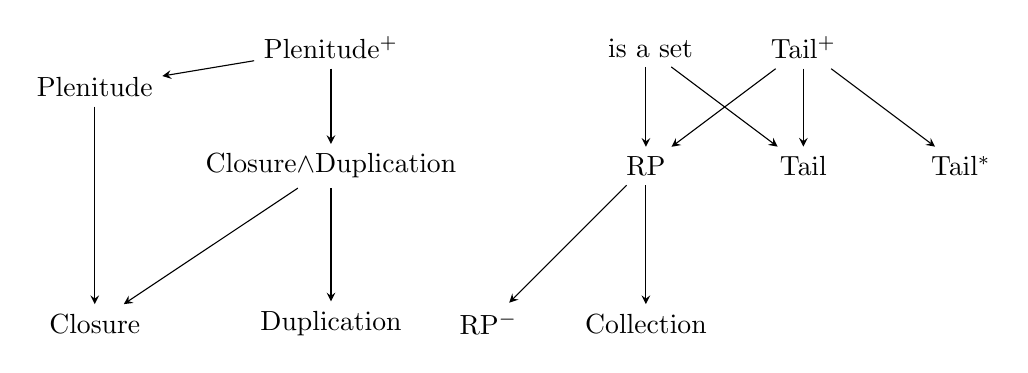
\begin{tikzpicture}
\begin{scope}[every node/.style={}]
    \node (B) at (5, 1.5){RP};
    \node (C) at (-2,2.5) {Plenitude};
        \node (D) at (1,3) {Plenitude$^+$};


          \node (G) at (3, -0.5) {RP$^-$};

    \node (H) at (1, 1.5) {\textup{Closure$\land$Duplication}};
    \node (I) at (5, -0.5) {Collection};

    \node (O) at (1, -0.5) {Duplication};
      \node (F) at (-2, -0.5) {Closure};


    \node (T) at (5, 3) {$\A$ is a set};
    \node (R) at (7, 3) {Tail$^+$};
    \node (S) at (7, 1.5) {Tail};
      \node (U) at (9, 1.5) {Tail$^*$};
    
\end{scope}

\begin{scope}[>={stealth},
              every node/.style={fill=white,circle},
              every edge/.style={draw=black}]
 
    \path [->] (T) edge (B);
    \path [->] (T) edge (S);
    \path [->] (D) edge (C);
    \path [->] (D) edge (H);
     \path [->] (C) edge (F);
    \path [->] (B) edge (I);
    \path [->] (B) edge (G);

    \path [->] (R) edge (S);
\path [->] (R) edge (U);
    \path [->] (R) edge (B);
    \path [->] (H) edge (O);
    \path [->] (H) edge (F);
\end{scope}
\end{tikzpicture}
\caption{Implication diagram in $\ZFUR$}
\label{ZFUdiagram}
\end{figure}
\FloatBarrier 
\noindent It is still unknown if the diagram is complete in $\ZFUR$. I shall prove several independence results in the next subsection and summarize some key open questions at the end of this chapter. 

To show Diagram \ref{ZFUdiagram} holds in $\ZFUR$, we utilize the following theorem proved in \cite{HamkinsForthcoming-HAMRIS}.

\begin{theorem}[\cite{HamkinsForthcoming-HAMRIS}]\label{homo->RP}
$\ZFUR$ + Collection + $\ACA$ $\vdash$ RP. \qed
\end{theorem}
\noindent Note that if $\A$ is a set, then the usual proof of RP in ZF works; and RP implies Collection by Proposition \ref{RP->Collection}. So it remains to show the following.
\begin{theorem}\label{thm:Plenitude+->duplication}
Over $\ZFUR$,
\begin{enumerate}
    \item Tail$^+$ $\rightarrow$ RP;
    \item Plenitude$^+$ $\rightarrow$ Duplication.
\end{enumerate}
\end{theorem}
\begin{proof}
(1) Assume Tail$^+$. Consider a well-ordered tail for $\emptyset$. Then every set of urelements can be injectively mapped to this set of urelements, so $\ACA$ holds. Then it follows from Lemma \ref{tail->collection} that Collection holds, so we can apply Theorem \ref{homo->RP}.



(2) Assume Plenitude$^+$. Suppose \textit{for reductio} that some $A \subseteq \A$ cannot be duplicated. Consider any ordinal $\alpha$. Then there is a bijection $f$ from $A \times \alpha$ to some set of urelements $B$. It follows that for every $\beta < \alpha$, $A \cap f[A_\beta]$ is non-empty, where $A_\beta = A \times \{\beta\}$, which produces an injection from $\alpha$ to $P(A)$. This shows that every ordinal can be mapped injectively into $P(A)$, contradicting Hartog's Theorem.
\end{proof}


\subsection{Permutation models}
 Now I proceed to prove some independence results concerning Diagram \ref{ZFUdiagram} by constructing suitable models. Note that the $V\llbracket X \rrbracket$-construction in Definition \ref{barwiseinterpretation1} is not flexible enough for such task. Firstly, $V\llbracket X \rrbracket$ always satisfies Collection (Theorem \ref{thm:V[X]modelsZFU}), while we wish to show that, for instance, Plenitude does not imply Collection over $\ZFUR$. Secondly, it folllows from Theorem \ref{thm:ACholdsViffACholdsinV[X]} that if $\ACA$ fails in $V\llbracket X \rrbracket$, then AC fails for the pure sets of $V\llbracket X \rrbracket$. But we may wish to construct models where AC only fails \textit{outside} $V$. The method I shall utilize is a combination of the $U^\I$-construction in Definition \ref{smallkernelmodel} and the technique of \textit{permutation models} due to Fraenkel \cite{fraenkel1922begriff}, Mostowski \cite{mostowski1939begriff}, and Specker \cite{Specker1957-SPEZAD}. Since the standard text book on permutation models \cite{jech2008axiom} only considered permutation models with a \textit{set} of urelements, here I shall consider a more general construction allowing a proper class of urelements.
\begin{definition}[$\ZFCUR$]\label{permutationmodeldef}
Let $A$ be a set of urelements and $\G_A$ be a \textit{group} of permutations of $A$. For every $x$, define $sym(x) = \{\pi \in \G_A : \pi x = x\}$; if $x$ is a set, define $fix(x) = \{\pi \in \G_A : \pi y = y \text{ for all } y\in x \}$. A \textit{normal filter} $\F$ on $\G_A$ is a non-empty set of subgroups of $\G_A$ which contains $sym(a)$ for every urelement $a \in \A$ and is closed under supergroup, finite intersection, and conjugation (i.e., for all $\pi \in \G_A$ and $H \in \F$, $\pi H \pi^{-1} \in \F$). An object $x$ is \textit{symmetric} (with respect to $\F$) if $sym(x) \in \F$. The \textit{permutation model} $W$, determined by $A$, $\G_A$, and $\F$, is the class of all \textit{hereditarily symmetric} objects, i.e., $W = \{x \in U : x \text{ is symmetric} \land x \subseteq W\}$.
\end{definition}
\noindent If $x$ is symmetric, then so is $\pi x$ for every $\pi \in \G_A$ because $sym(\pi x) = \pi \circ sym(x) \circ \pi^{-1}$ and $\F$ is closed under conjugation. By an $\in$-induction, it follows that if $x \in W$, then $\pi x \in W$ for every $\pi \in \G_A$. Therefore, every $\pi \in \G_A$ is an automorphism of $W$.
\begin{theorem}[$\ZFCUR$]\label{fundamentalthmPM}
Let $A$, $\G_A$ and $\F$ model be as in Definition \ref{permutationmodeldef}. And let $W$ be the resultant permutation model. Then 
\begin{enumerate}
    \item $W \models \ZFUR$;
    \item $W \models$ Collection if $U \models$ Collection.
\end{enumerate}
\end{theorem}
\begin{proof}
(1) Since $W$ is transitive and contains all the pure sets, Extensionality, Foundation, and Infinity all hold in $W$, and AC holds for the pure sets of $W$. Union holds in $W$ because for any set $x \in W$, $sym(x) \subseteq sym(\bigcup x)$. If $x, y \in W$, $sym(x) \cap sym(y) \subseteq sym(\{x, y\})$, so $W$ satisfies Pairing.

\textit{Powerset.} Let $x \in W$ be a set. It suffices to show that $P^W(x) = \{y \in W : y \subseteq x\}$ is symmetric. If $\pi \in sym(x)$ and $y \in P^W(x)$, then $\pi y \subseteq x$ and $\pi y \in W$, so $\pi y \in P^W(x)$. This shows that $sym(x) \subseteq sym(P^W(x))$, and hence $P^W(x)$ is symmetric.

\textit{Separation.} Let $x \in W$ be a set. It suffices to show that the set $v = \{y \in W : y \in x \land \varphi^W(y, u)\}$ is symmetric, where $u$ is a parameter in $W$. If $\pi \in sym(x) \cap sym(v)$ and $y \in v$, it follows that $\pi y$ is in $W \cap x$ and $\varphi^W(\pi y,x,u)$ since $\pi$ is an automorphism of $W$. So $sym(x) \cap sym(v) \subseteq sym(v)$ and hence $v$ is symmetric.

\textit{Replacement.} Suppose that $W \models \forall x \in w \exists ! y \varphi(x, y, u)$, where $w, u \in W$. Let $v = \{y \in W : \exists x \in w \ \varphi^W(x, y, u)\}$, which is a set by Replacement in $U$. It suffices to show that $sym(w)\cap sym(u) \subseteq sym(v)$. If $\pi \in sym(w)\cap sym(u)$ and $y \in v$, then $\varphi^W(x, y, u)$ for some $x \in w$ and so $\varphi^W(\pi x, \pi y, u)$ for some $\pi x \in w$; thus, $\pi y \in v$ and hence $sym(w)\cap sym(u) \subseteq sym(v)$.

(2) Suppose that $U \models$ Collection and that $W \models \forall x \in w \exists y \varphi(x, y, u)$ for some $x, u \in W$. So in $U$ there is a $v$ such that $\forall x \in w \exists y \in v (y \in W \land \varphi^W(x, y, u))$. Let $B = A \cup ker(v)$. $B \in W$ because every $\pi \in \G_\A$ point-wise fixes all urelements outside $A$. Thus, $W \models \forall x \in w \exists y \in V(B) \ \varphi(x, y, u)$, and this suffices for Collection to hold in $W$ by Proposition \ref{weakcollection}. 
\end{proof}
\begin{definition}\label{Gnormalideal}
Given an $A\subseteq\A$ and a group $\G_A$ of permutations of $A$, $I \subseteq P(A)$ is a $\G_A$-\textit{normal ideal} on $A$ if and only if
\begin{enumerate}
    \item $A \notin I$;
    \item if $E_1, E_2 \in I$, then $E_1 \cup E_2 \in I$; 
    \item if $E_1 \in I$ and $E_2 \subseteq E_1$, then $E_2 \in I$;
    \item for every $a \in A$, $\{a\} \in I$;
    \item for every $E \in I$ and $\pi \in \G_A$, $\pi E \in I$.
\end{enumerate}
\end{definition}
\noindent If $I$ is a $\G_A$-normal ideal on $A$, it is not hard to verify that $$\F = \{ H \subseteq \G_A: H \text{ is a subgroup of }\G_A \text{ and } fix(E) \subseteq H \text{ for some } E \in I \}$$ is a normal filter on $\G_A$. Thus, in this case $A$, $\G_A$, and $I$ will generate a permutation model $W$. For every $x$ in such $ W$, there will be some $E \in I$, called a \textit{support} of $x$, such that $fix(E) \subseteq sym(x)$. This concludes the basic setup of permutation models. 

\begin{example}[The Basic Fraenkel Model]\label{exp:BasicFModel}
Let $U$ be a model of ZFCU in which $\A$ is a countably infinite set, $\G_\A \in U$ be the group of all permutations of $\A$, and $I$ be the ideal of finite subsets of $\A$. In the resulting permutation model $W$, although $\A$ is still the set of all urelements, no set of urelements is equinumerous with $\omega$ because any injection from $\omega$ to some $A\subseteq\A$ would have a finite support, which is impossible.
\end{example}
\begin{corollary}
Assume the consistency of ZF. There is a model of $\ZFUR$ in which 
\begin{enumerate}
    \item $\A$ is a set;
    \item Closure fails;
    \item Tail$^*$ fails.
\end{enumerate}
\end{corollary}
\begin{proof}
Consider the Basic Fraenkel Model.
\end{proof}

\subsection{Independence results}
Many implications in Diagram \ref{ZFCUdiagram} fail in $\ZFUR$. In particular, I shall prove that over $\ZFUR$,
\begin{enumerate}
    \item Plenitude $\nrightarrow$ (Duplication $\lor$ Collection);
    \item Tail$^*$ $\nrightarrow$ (Collection $\lor$ Tail);
    \item (Plenitude $\land$ Duplication) $\nrightarrow$ Collection;
    \item (RP $\land$ DC$_\omega$-scheme) $\nrightarrow$ Homogeneity holds over some $A\subseteq\A$.
\end{enumerate}
\begin{theorem}\label{plenitudenvdashcollection}
Assume the consistency of ZF. There is a model of $\ZFUR$ in which 
\begin{enumerate}
    \item Plenitude holds;
    \item Collection fails;
    \item Duplication fails.
\end{enumerate}
\end{theorem}
\begin{proof}
Let $U$ be a model of ZFCU + Plenitude. In $U$, fix a countable set of urelements $A \subseteq \A$ and enumerate it with $\omega \times \omega$. So $A = \bigcup_{n<\omega} A_n$, where each row $A_n$ is an infinitely countable sequence of urelements. Let $\G_A$ be the group of permutations of $A$ that preserve each $A_n$, i.e, a permutation $\pi$ of $A$ is in $\G_A$ just in case $\pi A_n = A_n$ for every $n<\omega$. Let $I = \{E \subseteq A : E \text{ is finite} \}$, which is a $\G_A$-normal ideal on $A$. Now let $W$ be the permutation model generated by $A$, $\G_A$ and $I$. By Theorem \ref{fundamentalthmPM}, $W \models \ZFUR$ + Collection.



To get the failure of Collection, we go to an inner model of $W$ by using the construction in Definition \ref{normalideal}. Since the sequence $\<A_n : n <\omega>$ is in $W$, say a $B\subseteq \A$ \textit{is finitely contained in} $A$ if $A \cap B$ is a subset of the union of finitely many $A_n$. Define $\I = \{B \subseteq \A : B  \text{ is finitely contained in } A \}$, which is an $\A$-ideal. This produces an inner model $W^\I = \{ x \in W : ker(x) \in \I\}$, and by Theorem \ref{smallkernelmodel}, $W^\I \models \ZFUR$. 

Note that if $B$ is a set of urelements in $W^\I$ that is disjoint from $A$, then $B$ is well-orderable in $W^\I$ because every $\pi \in G_A$ point-wise fixes $B$, so its well-ordering in $U$ is preserved through the constructions. It follows that  $W^\I \models$ Plenitude since in $U$ we can find arbitrarily large sets of urelements disjoint from $A$.
\begin{lemma}\label{amorphous}
In $W^I$, each $A_n$ is \textit{amorphous}, i.e., it is infinite but is not a union of two disjoint infinite sets.
\end{lemma}
\begin{proof}
Suppose for \textit{reductio} that $A_n = B_1 \cup B_2$ for two infinite disjoint sets $B_1$, $B_2$ in $W^\I$. Let $E_1 \in I$ be a support of $B_1$. Since both $B_1 \setminus E_1$ and $B_2 \setminus E_1$ are non-empty, we can pick an urelement from each of them and let $\pi$ be a permutation in $\G_A$ that only swaps these two urelements. It follows that $\pi B_1 \neq B_1$ and $\pi \in fix(E_1)$, contradicting the fact that $E_1$ supports $B_1$.\end{proof}

\begin{lemma}
$W^\I \models \neg$Collection.
\end{lemma}
\begin{proof}
The following holds in $W^\I$ since $W^\I$ contains $A_0 \cup ... \cup A_{n-1}$ for each $n$.
\begin{align}
    \forall n < \omega \ \exists D \subseteq\A \ (D \text{ is a union of } n \text{ disjoint amorphous sets}).
\end{align}
Suppose \textit{for reductio} that Collection holds in $W^\I$. Then there is a set $v \in W^\I$ such that
\begin{align}
    \forall n < \omega \ \exists D \in v \ (D \subseteq \A \land D \text{ is a union of } n \text{ disjoint amorphous sets}).
\end{align}
And $ker(v) \cap A$ is contained in an $m$-block of $A_n$, $A_{n_1} \cup ... \cup A_{n_m}$, for some finite number $m$. By (2.2), there is a set of urelements $D \in v$ such that $D = D_1 \cup ... \cup D_{m+1}$, where $D_1, ..., D_{m+1}$ are disjoint amorphous sets. For each $k \leq m+1$, $D_k \cap A$ must be infinite because any set of urelements disjoint from $A$ is well-orderable in $W^\I$. Since $D_k \cap A = D_k \cap (A_{n_1} \cup ... \cup A_{n_m})$, it follows that for each $k \leq m+1$, there is an $l \leq m$ such that $D_k \cap A_{n_l}$ is infinite. However, no two $D_k$ and $D_{k'}$ can have an infinite intersection with the same $A_{n_l}$ by Lemma \ref{amorphous}. This is a contradiction because it amounts to having an injection from $m+1$ to $m$.
\end{proof}
It remains to show that $W^\I \models$ $\neg$Duplication. It suffices to show that in $W^\I$, for each $A_n$ and any infinite set of urelements $B$, if $B \cap A_n$ is finite, then there is no injection from such $B$ to $A_n$. Suppose \textit{for reductio} that $f$ is an injection from $B$ to $A_n$ in $W^\I$. Let $E \in I$ be a support of $f$. Then there must be two urelements $a, b \in A_n \setminus (E\cup B)$. Let $\pi \in fix(E)$ swap only $a$ and $b$. It then follows that $f(b) = \pi f(a) = f(a)$, contradicting the injectivity of $f$. 
\end{proof}

\begin{theorem}
Assume the consistency of ZF. There is a model of $\ZFUR$ in which 
\begin{enumerate}
    \item Tail$^*$ holds;
    \item Collection fails;
    \item Tail fails.
\end{enumerate}
\end{theorem}
\begin{proof}
Let $U$ be a model of ZFCU + $\A \sim \omega_1$, where $\A$ is enumerated with $\omega \times \omega_1$. So $\A = \bigcup_{n < \omega} A_n$, where each row $A_n$ is uncountable. Let $G_\A$ be the group of permutations of $\A$ that preserve each row $A_n$ and $I = \{E \subseteq \mathcal{A} : E \text{ is countable} \}$. This generates a permutation model $W$. In $W$, define $\I = \{B \subseteq \mathcal{A} : B \text{ is finitely contained in } \A\}$.
\begin{lemma}\label{noomega1set}
In $W^\I$, no $A_n$ contains two disjoint subsets that are both uncountable. Hence, in $W^I$ there is no set of urelements of size $\omega_1$.
\end{lemma}
\begin{proof}
 Suppose \textit{for reductio} that in $W^\I$, $B_1, B_2 \subseteq A_n$ are disjoint and uncountable. Let $E \in I$ be a support of $B_1$. Then we can pick an urelement from each $B_1 \setminus E$ and $B_2 \setminus E$ respectively. A permutation that swaps only these two urelements will then fix $B_1$, which is a contradiction.
\end{proof}
\noindent Note that for each $n$, every countable subset of $A_n$ remains countable in $W^\I$. So for every set of urelements $B \in W^\I$, we can always find $\omega$-many urelements outside the finite block containing $B$. It follows from Lemma \ref{noomega1set} that Tail$^*$ holds in $W^\I$.

Suppose \textit{for reductio} that Collection holds in $W^\I$. Since for every $n<\omega$, there is a set of urelements that is a disjoint union of $n$ uncountable sets, it follows that there is some $v$ such that for every $n<\omega$, there is a set of urelements $D \in v$ that is a disjoint union of $n$ uncountable sets. Then $ker(v) \subseteq A_{n_1} \cup .... \cup A_{n_m}$ for some $m < \omega$. And there is some $D\subseteq A_{n_1} \cup  ....\cup A_{n_m}$ such that $D = D_1 \cup ... D_{m+1}$, where for each two $k, l \leq m+1$, $D_k$ and $D_l$ are disjoint and uncountable. For each $k \leq m+1$, there is a $l \leq m$ such that $D_k \cap A_{n_l}$ is uncountable; but no two $D_k$ and $D_{k'}$ can have an uncountable intersection with the same $A_{n_l}$ by Lemma \ref{noomega1set}. This is a contradiction, so Collection fails in $W^\I$. 

To see that Tail fails in $W^\I$, fix an $A_n$. For any $B$ that is disjoint from $A_n$, there is a row $A_m$ that is disjoint from $B \cup A_n$. But it is clear that there cannot be an injection in $W^\I$ from $A_m$ to $B$. \end{proof}

\begin{theorem}
Assume the consistency of ZF. There is a model of $\ZFUR$ in which 
\begin{enumerate}
    \item Plenitude holds;
    \item Duplication holds;
    \item Collection fails.
\end{enumerate}
\end{theorem}
\begin{proof}
Let $U$ be a model of ZFCU + Plenitude. In $U$, fix a set of urelements $A$ of size $\omega$ and enumerate it with $\omega \times \omega$, i,e, $A = \bigcup_{n<\omega} A_n$. We then identify each row $A_n$ with the rationals $\<\Q, <_\Q >$ such that $A_n = \{a^n_j : j \in \Q\}$. Define $\G_A$ as the following permutation group such that for every permutation $\pi$ of $A$,
\begin{itemize}
    \item [] $\pi \in \G_A$ if and only if there is an automorphism $\rho$ of $\<\Q, <_\Q>$ such that $\pi(a^n_j) = \pi (a^n_{\rho(j)})$ for every $n < \omega$ and $j \in \Q$.
\end{itemize}

\noindent That is, each $\pi \in \G_A$ follow a same automorphism of $\Q$ at each row $A_n$. Define $I = \{E \subseteq A : E \text{ is finite} \}$, which is a $\G_A$-normal ideal on $A$, and let $W$ be the permutation model generated by $A$, $\G_A$, and $I$. And as before, let $\I = \{B \subseteq \A : B \cap A \text{ is finitely contained in } A\}$. Plenitude holds in $W^\I$ because every set of urelements disjoint from $A$ is well-orderable in $W^\I$.
\begin{lemma}\label{Anareduplicates}
In $W^\I$, for every distinct $n, m <\omega$, $A_n$ and $A_m$ are duplicates.
\end{lemma}
\begin{proof}
Recall that two sets of urelements are said to be \textit{duplicates} if they are disjoint and equinumerous. It suffices to show that the bijection $f : A_n \rightarrow A_m$ that maps $a^n_i$ to $a^m_i$ for every $i \in \Q$ is symmetric. Consider any $\pi \in \G_\A$ and let $\rho$ be the automorphism of $\Q$ such that $\pi a^k_i = \pi a^k_{\rho i}$ for every $k < \omega$ and $i \in \Q$. For every $\<a^n_i, a^m_i> \in f$, $\<\pi a^n_i, \pi a^m_i > = \<a^n_{\rho i}, a^m_{\rho i}> \in f$. Therefore, $f$ is symmetric.
\end{proof}
\noindent For any set $B$ of urelements in $W^\I$, $B \setminus A$ can be easily duplicated outside $A$ because it is well-orderable and Plenitude holds. For $B \cap A$, since it is contained in an $m$-block of $A_n$ for some finite number $m$, we can find another disjoint $m$-block of $A_n$. By Lemma \ref{Anareduplicates}, it follows that these two blocks are duplicates, and in particular, $B \cap A$ will have a duplicate inside the disjoint block. This shows that Duplication holds in $W^\I$.

The failure of Collection in $W^\I$ will be proved through the following four lemmas.

\begin{lemma}\label{Anhasnoduplicates}
In $W^\I$, no $A_n$\footnote{Note that unlike in Theorem \ref{plenitudenvdashcollection}, $A_n$ is no longer amorphous: every $\pi \in \G_A$ that fixes $a^n_i$ will have to fix $\{a^n_j : j \leq i\}$ and $\{a^n_j : j > i\}$, making these two disjoint intervals symmetric.} contains a pair of infinite duplicates for any $n<\omega$. Hence, no infinite subset of $A_n$ is well-orderable. 
\end{lemma}
\begin{proof}
Suppose otherwise. Then in $W^\I$, there is some injection $f$ from $B$ to $B'$, where $B, B'$ are infinite duplicates and $B, B' \subseteq A_n$ for some $n$. Let $E \in I$ be a support of $f$. Since $E$ is finite, it follows that there must be some $a^n_i \in B \setminus E$ and $a^n_j \in B' \setminus E$ such that $f(a^n_i) = a^n_j$. Then we can find an open interval of $\Q$ that contains $j$ but no rational indexes that appeared in $E  \cup \{a^n_i\}$. Any non-trivial automorphism of $\Q$ that only moves points in this interval will generate a $\pi \in G_\A$. Clearly, $\pi \in fix(E \cup \{a^n_i\})$; so $f(a^n_i) = \pi a^n_j \neq a^n_j$, which is a contradiction.
\end{proof}
For any urelement $a^n_i \in A_n$, we say that a function $f$ \textit{vertically fixes} $a^n_i$ if $f (a^n_i) = a^m_i$ for some $m$.
\begin{lemma}\label{alignment}
 In $W^\I$, if $B\subseteq A_n$ and $B' \subseteq A_m$ are infinite, where $n \neq m$, then for every injection $f$ from $B$ to $B'$, $f$ vertically fixes infinitely many $a^n_i \in B$.
\end{lemma}
\begin{proof}
Let $E \in I$ be a support of $f$. We show that for every $a^n_i \in B \setminus E$, $f(a^n_i) = a^m_i$. Suppose \textit{for reductio} that $f(a^n_i) = a^m_j$ and $i \neq j$. Then we can find an interval of $\Q$ that contains $i$ but no rational indexes that have appeared in $E \cup \{a^m_j\}$, which will give us a $\pi \in fix(E \cup \{a^m_j\})$. But then $f(\pi a^n_i) = a^m_j$ and $\pi a^n_i \neq a^n_i$, contradicting the assumption that $f$ is injective.\end{proof}

For a set of urelements $B$, we say that it has a \textit{nice n-partition} if  there are $B_1, ... B_n$ such that 
\begin{itemize}
    \item [] (i) $B = B_1 \cup ... \cup B_n$;
    \item [] (ii) for each two $k, l \leq n$, $B_k, B_l$ are non-well-orderable duplicates.
\end{itemize}
\begin{lemma}\label{partition}
In $W^\I$, there is no set of urelements $B$ such that for every $n < \omega$, $B$ has a subset with a nice $n$-partition.
\end{lemma}
\begin{proof}
Suppose \textit{for reductio} that $B \in W^\I$ is such set. Then we may assume that $B \cap A \subseteq A_1, ..., A_n$ for some finite number $n$. Let $C \subseteq B$ be a set with a nice $n+1$-partition such that $C = C_1 \cup ... \cup C_{n+1}$, where for each two $k, l \leq n$, $C_k, C_l$ are non-well-orderable duplicates. And for each $1 \leq k < n+1$, let $f_k \in W^\I$ be a bijection from $C_k$ to $C_{k+1}$. Define an $(n+1)$-sequence of pairs $\<m_{1}, D_1, >, ..., \<m_{n+1}, D_{n+1}>$ by recursion as follows.
\begin{itemize}
   \item [] $m_1$ is the least number $\leq n$ such that $C_1 \cap A_{m_1}$ is infinite; and
    \item [] $D_1 = \{a \in C_1 \cap A_{m_1} : f_1  \text{vertically fixes } a \}$.
\end{itemize}   
Suppose that $\<m_{k-1}, D_{k-1}>$ has been defined. Then
 \begin{itemize}
    \item [] $m_{k}$ is the least number $\leq n$ such that $f_{k-1}[D_{k-1}] \cap A_{m_k}$ is infinite; and
    \item [] $D_{k} = \{ a \in f_{k-1} [D_{k-1}] \cap A_{m_k}: f_k \text{ vertically fixes } a\}$.
\end{itemize}
\begin{claim}
For each $k \leq n+1$, $m_k$ exists and $D_k \subseteq C_k$ is infinite. Hence, the sequence above is well-defined.
\end{claim}
\begin{claimproof}
First,  $m_1$ exists. For $C_1$ is non-well-orderable so $C_1 \cap A$ must be infinite, and since $C_1 \cap A \subseteq B \cap A \subseteq A_1 \cup ... \cup A_n$, it follows that $C_1 \cap A_m$ is infinite for some $m \leq n$ and hence $m_1$ exists. Second, observe that $D_1$ is infinite. $f_1[C_1 \cap A_{m_1}]$ is non-well-orderable because $C_1 \cap A_{m_1}$ is by Lemma \ref{Anhasnoduplicates}; so infinitely many urelements in $f_1[C_1 \cap A_{m_1}]$, which is a subset of $C_2$, live in $A$ and hence in some $A_l$, where $l \leq n$. Since $C_1$ and $C_2$ are disjoint, $l \neq m_1$ by Lemma \ref{Anhasnoduplicates}. This means that $f_1$ moves infinitely many urelements in $C_1 \cap A_{m_1}$ to another row $A_l$, and by Lemma \ref{alignment}, $f_1$ must vertically fix infinitely many urelements in  $C_1 \cap A_{m_1}$. Therefore, $D_1$ is infinite.

Now suppose that $\<m_{k-1}, D_{k-1}>$ exists and $D_{k-1} \subseteq C_{k-1}$ is infinite. Then $f_{k-1}[D_{k-1}]$, which is a subset of $C_{k} \cap A$, must have an infinite intersection with some $A_l$ for $l \leq n$. Hence $m_k$ exists. By the same reasoning as in the last paragraph, it follows that $f_k$ must vertically fix infinitely many urelements in $f_{k-1}[D_{k-1}] \cap A_{m_k}$, and hence $D_k$ is infinite.
\end{claimproof}

\begin{claim}
For every natural number $l > 0$, whenever $k, k+l \leq n+1$ for some natural number $k$, then for every $a^{m_{k+l}}_i \in D_{k+l}$, there is some $a^{m_k}_i \in D_k$ such that $a^{m_{k+l}}_i = f_{k+l-1} \circ ...\circ f_k(a^{m_k}_i)$.
\end{claim}
\begin{claimproof}
By an easy induction on $l$. When $l = 1$, the claim follows by the definition of $D_k$. Suppose it holds for $l - 1 (> 0)$ and consider $k, k+l \leq n+1$. For every $a^{m_{k+l}}_i \in D_{k+l}$, there is an $a^{m_{k+l-1}}_i \in D_{k+l-1}$ such that $f_{k+l-1}(a^{m_{k+l-1}}_i) = a^{m_{k+l}}_i$. By the induction hypothesis, there is an  $a^{m_k}_i \in D_k$ such that $a^{m_{k+l-1}}_i = f_{k+l-2} \circ ...\circ f_k(a^{m_k}_i)$, and so the claim follows.\end{claimproof}


It then follows from the claim that if $k < k' \leq n+1$, then $m_k \neq m_k'$. Otherwise, by the previous claim we can find a $a^{m_{k}}$ in both $D_k$ and $D_k'$, which are disjoint. However, this is a contradiction, because for each $k \leq n+1$, $m_k \leq n$. The lemma is thus proved. \end{proof}


Now suppose \textit{for reductio} that Collection holds in $W^\I$. In $W^\I$, we have 
\begin{align}
     \forall m < \omega \exists B \subseteq \A (B \text{ has a nice } m \text{-partition}).
\end{align}
This is because the union of any $m$-block of $A_n$ has has a nice $m$-partition, since each pair of $A_n$ are duplicates by Lemma \ref{Anareduplicates}. Then by Collection, 
\begin{align}
   \exists v \forall m < \omega \exists B \in v (B \subseteq \A \land B \text{\ has a nice } m\text{-partition}).
\end{align}
This means that for every $m$, $ker(v)$ has a subset with a nice $m$-partition, which contradicts Lemma \ref{partition}. This completes the proof of the theorem. \end{proof}

The next theorem explains why all the $\ZFCUR$ arguments fail without choice: homogeneity, which is crucial for those arguments to go through, may fail globally when $\ACA$ is not assumed.
\begin{theorem}\label{thm:RPdoesnotproveHomogeneity}
Assume the consistency of ZF. There is a model of $\ZFUR$ in which
\begin{enumerate}
    \item the DC$_\omega$-scheme holds;
    \item RP holds;
    \item homogeneity holds over no set of urelements.
\end{enumerate}
\end{theorem}
\begin{proof}
Let $U$ be a model of ZFCU in which $\A$ is a set of size $\omega_1$  and enumerate $\A$ with $\omega_1 \times \omega_1$, i.e., $\A = \bigcup_{\alpha < \omega_1} A_\alpha$, where each row $A_\alpha$ is uncountable. Let $G_\A$ be the group of permutations of $\A$ that preserve $A_\alpha$ for each $\alpha < \omega_1$ and $I = \{E \subseteq \mathcal{A} : E \cap A_\alpha \text{ is countable for each } \alpha < \omega_1\}$. This generates a permutation model $W$. In $W$, let $\I = \{B \subseteq \mathcal{A} : B \text{ is countably contained in } \A\}$.


As before, it follows that in $W^\I$, for any $\alpha, \beta <\omega_1$ such that $\alpha \neq \beta$, there is no injection from $A_\alpha$ to $A_\beta$. The next lemma says that every permutation of $\A$ that only swaps some $A_\alpha$ fixes $W^\I$.

 \begin{lemma}\label{Wfix}
In $U$, if $\sigma$ is a permutation of $\mathcal{A}$ such that for every $\alpha < \omega_1$, $\sigma A_{\alpha} = A_{\beta}$ for some $\beta$ (consequently,  $A_{\alpha} = \sigma A_{\gamma}$ from some $\gamma$), then $\sigma (W^\I) = W^\I$. 
\end{lemma}
\begin{proof}
Since $W^\I$ is a class of $U$ defined by $\mathcal{G}_\A, \ I$, and $\I$, it suffices to show that they are all fixed by $\sigma$. If $\pi \in \G_\A$, then for every $A_\alpha$, since $A_\alpha = \sigma A_\beta$ for some $\beta$ and $\pi A_\beta = A_\beta$, by automorphism it follows that $(\sigma \pi) (\sigma A_\beta) = \sigma A_\beta$; so $(\sigma \pi )A_\alpha = A_\alpha$ and hence $\sigma \pi \in \mathcal{G}_\A$.\footnote{Note here $\sigma \pi$ is not $\sigma \circ \pi$ but $\{\langle \sigma a, \sigma (\pi a) \rangle : a \in \mathcal{A} \rangle\}$} This shows that $\sigma \mathcal{G}_\A = \mathcal{G}_\A$. If $E \in I$, then for every $A_\alpha$, since $A_\alpha = \sigma A_\beta$ for some $\beta$ and $E \cap A_\beta$ is countable, $\sigma E \cap A_\alpha$ is countable and hence $\sigma E \in I$. Therefore, $\sigma I= I$. Similarly, if $B$ is contained in countably many $A_\alpha$, then so is $\sigma B $. Hence, $\sigma \I= \I$ and the lemma is proved.
\end{proof}
\begin{lemma}
$W^\I \models $ DC$_\omega$-scheme.
\end{lemma}
\begin{proof}
Suppose that in $W^\I$, $\varphi(x, y, u)$ defines a relation without terminal nodes. By the DC$_\omega$-scheme in $U$, there is an infinite sequence $\<x_n : n<\omega>$ in $U$ such that $x_n \in W^\I$ and $W^\I \models \varphi(x_n, x_{n+1}, u)$ for every $n$. By AC in $U$, for each $n$ we can choose an $E_n$ which is a support of $x_n$. Then $\bigcup_{n < \omega} E_n$ is in $I$, and as $\bigcup_{n < \omega} E_n $ supports $\langle x_n : n < \omega \rangle$, the sequence is also in $W$. Furthermore, since each $ker(x_n)$ is in $\I$ and $\I$ is countably closed, it follows that the kernel of this sequence is also in $\I$. Therefore, the  DC$_\omega$-scheme holds in $W^\I$. 
\end{proof}

\begin{lemma}
$W^\I \models $ Collection.
\end{lemma}
\begin{proof}
Suppose that $W^\I\models \forall x \in w \exists y \varphi(x, y, u)$ for some $w, u \in W^\I$. Let $\{ A^1_{n} : n < \omega \}$ be a countable block containing $ker(w) \cup ker(u)$ and $\{ A^2_n : n < \omega \}$ be a countable block that is disjoint from each $A^1_{n}$. Set $A = \bigcup_{n<\omega} (A^1_n \cup A^2_n )$. It suffices to show that $W^\I\models \forall x \in w \exists y \in V(A) \varphi(x, y, u)$. Suppose that $x \in w$ and fix some $y \in W^\I$ such that $W^\I \models \varphi(x, y, u)$. Let $\{ A^3_n : n <\omega\}$ be another disjoint countable block that contains $ker(y) \setminus A$. Back in $U$, find another block $\{A^4_n : n <\omega \}$ disjoint from all of these three blocks. Using AC in $U$ we can define a permutation $\sigma$ of $\mathcal{A}$ as follows. Let $\sigma$ move each $A^2_n$ to $A^2_{2n}$, each $A^3_n$ to $A^2_{2n+1}$, each $A^4_{2n}$ to $A^3_n$ and each $A^4_{2n+1}$ to $A^4_n$. By Lemma \ref{Wfix}, it follows that $\sigma (W^\I) = W^\I$. Since $ W^\I \models \varphi(x, y, u)$ and $\sigma$ fixes $x$ and $u$, it follows that $W^\I \models \varphi(x, \sigma y, u) \land \sigma y \in  V(A)$.\end{proof}
By Theorem \ref{collection+dc->rp}, the last two lemmas jointly imply that $W^\I \models $ RP. Finally, for every $A \subseteq \A$ in $W^\I$, there will be some $A_\alpha$ and $A_\beta$ such that $A$, $A_\alpha,$ and $A_\beta$ are pair-wise disjoint. But there is no injection from $A_\alpha$ to $A_\beta$. Therefore, homogeneity holds over no set of urelements in $W^\I$, which completes the proof.\end{proof}



\subsection{Open questions}
\begin{question}
Is Diagram \ref{ZFUdiagram} complete over $\ZFUR$? In particular, does $\ZFUR$ prove any of the following?
\begin{enumerate}
    \item Plenitude$^+ \rightarrow$ Collection.
    \item Tail $\rightarrow$ Collection.
    \item Collection $\rightarrow$ RP$^-$.
    \item RP$^- \rightarrow$ Collection.
\end{enumerate}
\end{question}
\noindent My conjecture is that $\ZFUR$ + Collection cannot prove RP$^-$ (and therefore RP). This conjecture has several implications from a philosophical perspective. Some may view this result as another compelling evidence in support of the reflection conception of sets, as it highlights the limitations of the iterative conception in the choiceless context. Thus, the iterative conception may be seen as an incomplete picture of sets. Conversely, the independence of RP could lead others to question the reflection conception in the context of urelements. And the fact that ZFCU proves RP suggests that RP is a form of choice principle, which may not be natural in urelement set theory. Furthermore, an alternative perspective is that these independence results demonstrate another instance of axiomatic freedom, emphasizing that there may not necessarily be a ``correct" system. 